\documentclass[10pt,a4paper]{article}

\usepackage{a4wide}
\usepackage{amsmath}
\usepackage{amssymb}
\usepackage{mathspec}
\setallmainfonts[Ligatures=TeX]{Linux Libertine O}

%\usepackage{txfonts}
% \usepackage{microtype}

% \usepackage{a4wide}
% \usepackage{epsfig}
\usepackage{graphicx}
\usepackage{caption}
\usepackage{subcaption}
% \usepackage{moreverb}
% \usepackage{hyperref}

\usepackage{url}

\usepackage[affil-it]{authblk}
\usepackage[margin=2.5cm]{geometry}

\title{A short report on the generation of synthetic microstructures of WC-Co cemented carbides}
\author{Sven~A.~E. Johansson}
\affil{Department of Applied Physics, Chalmers University of Technology, SE-412 96 G{\"o}teborg, Sweden\\
Chalmers industriteknik, Sven Hultins gata 9D, SE-412 88 G{\"o}teborg, Sweden}

\begin{document}

\maketitle

\begin{abstract}
	A method of generating synthetic microstructures of WC-Co cemented carbides is presented. The method is based on a voxel-representation of the simulation volume. WC grains are modeled as truncated triangular prisms with predefined shape factors. The grains are subject to uniformly random rigid rotations and then inserted randomly into the simulation volume while attempting to minimize grain overlap. To obtain realistic microstructures, a Potts simulation is performed as a last stage to remove unphysical artefacts due to remaining grain overlap. The final structures appear realistic to the naked eye. As a statistical test, the contiguity vs. Co fraction curve shows good agreement with published experimental measurements for small Co volume fractions.
\end{abstract}


% {\noinden}
% Sven~A.~E. Johansson\\
% \textit{Department of Applied Physics, Chalmers University of Technology, SE-412 96 G{\"o}teborg, Sweden}
% }

\section{Introduction}
This is a short report on an effort to create a computer model of a three-dimensional (3D) microstructure resembling typical microstructures of fully-dense conventionally sintered WC-Co cemented carbides. The model is supposed to be used in finite-element method (FEM) modeling of WC-Co with cohesive zone models for WC/WC and WC/Co boundaries. The aim is to formulate a model that adequately reproduces the most important microstructural parameters in the WC-Co system. These include the volume fractions of the respective phases,  representative WC grain shapes,  WC grain size distributions, and the contiguity of the carbide phase \cite{Ex79,LaMi14}.

To our knowledge, prior work in generating a 3D synthetic microstructure of WC-Co is restricted to the paper of Magin and G{\'e}rard \cite{MaGe09}, who used CAD software to model the WC-Co structure. In their work, representative WC crystals of random rotation were randomly distributed in a Co binder. However, the grain structure of WC was not retained in their model, reducing their model to effectively two large (although complex) interpenetrating bodies of WC and Co. %A clear disadvantage with using CAD software is the computational complexity which excludes the possibility of iteratively changing the model structure with respect to its statistical properties.

The microstructure analysis software Dream3D \cite{GrJa14,Dream3D} has a module for generating synthetic microstructures based on a number of input statistics such as grain size, shape and neighbor distributions. It is based on a voxel-representation of volume, where shapes (ellipsoids, cylinders, cube octahedron) representing different grains are inserted in a random way while simultaneously trying to satisfy the given goal statistics. However, none of the grain shapes available in Dream3D resembles the typical triangular prism shape of WC grains sintered in liquid Co.

To allow full control of the microstructure generation, it was decided to write new separate code, named CCBuilder, for the WC-Co structure using the same kind of voxel representation as in Dream3D. Dream3D is a promising piece of software as it includes e.~g. functionality for surface meshing. Therefore, the output data structure of CCBuilder is made fully compatible with Dream3D data files to allow importing data into Dream3D for further processing.

\subsection{Microstructural parameters}
\label{subsec:microstructural_param}
Among the microstructural parameters that we aim to reproduce are volume fraction of WC and Co, $v_\text{WC}$ and $v_\text{Co}$, respectively ($v_\text{WC}+v_\text{Co}=1$). The contiguity $C$ of the carbide phase is important as it relates grain boundary $A_\text{gb}$ and phase boundary $A_\text{pb}$ areas according to \cite{Ex79,LaMi14}
\begin{equation}
	C = \frac{2 A_\text{gb}}{2 A_\text{gb} + A_\text{pb}}.
\end{equation}
A factor 2 is inserted in front of $A_\text{gb}$, since the contiguity is a measure of the degree of connection of one WC grain to other WC grains.

Another important parameter is the typical WC grain shape. The morphology of WC grains has been analyzed in a series of papers \cite{ChWaAlLa05,ChWaLaAl07,LaAlChWa08}, and the truncated triangular prism has been identified as the equilibrium WC shape in a Co surrounding. Its geometry is defined in e.~g. Ref.~\cite{ChWaLaAl07}. The truncation factor is given by
\begin{equation}
	r = \frac{a_\text{short}}{a_\text{long}}
\end{equation}
and the elongation factor
\begin{equation}
	k = \frac{t}{h}
\end{equation}
with $a_\text{short}$, $a_\text{long}$, $t$ and $h$ defined in Figure~\ref{fig:tt}. The equilibrium $r$ and $k$ values depend on the C chemical potential, which in turn depends on temperature and alloy composition. Experimental $r$ and $k$ values are reported in Ref.~\cite{LaAlChWa08}.

\begin{figure}
	\begin{center}
		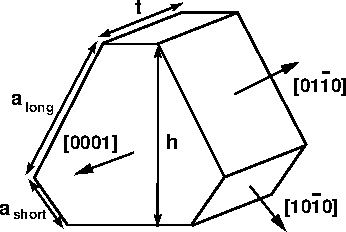
\includegraphics[width=.3\columnwidth]{Truncated_triangle_drawing/tt_drawing}
	\end{center}
	\caption{\label{fig:tt} The geometry of the truncated triangular prism from \cite{ChWaLaAl07}.}
\end{figure}

\section{CCBuilder}
For simplicity, CCBuilder is mainly written in Python with computationally extensive functions implemented in Cython \cite{Cython}, which is a superset of the Python language which adds static type declarations. This allows automatic conversion of Cython code into C code, which can be compiled and optimized to native binaries. If the Cython code is carefully written, i.~e. all variables are typed, contents of arrays are accessed through C pointers, bounds checks are disabled etc., the produced binares have performance fully on par with ``hand-written'' C code. The CCBuilder source code is available on GitHub \cite{CCBuilder}.

In CCBuilder, the volume considered is a cube of side $L$ divided into $M$ divisions giving a total of $M^3$ voxels represented in an integer array. Each voxel is assigned an integer $i$ representing the binder or the WC grain to which it belongs, where $i=1$ means Co binder and $i = 2, 3, \ldots$ means that the voxel belongs to WC grain number $i-2$ (numbered from $0$). The generation algorithm starts by initializing the volume as a pure binder, i.~e. all ones. The volume is then gradually filled with WC grains of predefined shapes.

The basic WC shape defined in CCBuilder is a truncated triangular prism as defined in Section~\ref{subsec:microstructural_param}. In CCBuilder, a list of prisms is generated by the function \verb|prepare_triangles|. The prisms are generated with $r$ and $k$ drawn from uniform random distributions $[r_\text{min},r_\text{max}]$ and $[k_\text{min},k_\text{max}]$, respectively. The volume of each grain is given by assigning a random equivalent sphere diameter $d_\text{eq}$ given from a uniform distribution $[d_\text{eq,min},d_\text{eq,max}]$ to each grain. The equivalent sphere diameter is related to the volume of grain $j$, $V_j$, by $4\pi/3 (d_\text{eq}/2)^3 = V_j$. $r$, $k$ and $d_\text{eq}$ are sufficient to fully define the shape and volume of the grain. To each grain, there is an associated rotation matrix, which defines the rotation state of the grain with respect to the $\hat{x}, \hat{y}, \hat{z}$ directions of the volume. The rotation matrix is drawn from a distribution of uniformly random rigid rotations using the algorithm of Brannon \cite{Br02}. An initial midpoint of each prism is drawn from a uniform distribution $[0,L]^3$. The number of generated prisms is controlled by a goal WC volume fraction $v_\text{WC, goal}$ and new grains are generated until $1/L^3 \sum_j V_j > v_\text{WC, goal}$, i.~e. a volume fraction that does not take into account the overlap between WC grains. Finally, the list of prisms is sorted in descending order of volume.

In the function \verb|make_voxel_indices|, a list of voxel indices is prepared for each grain. The generated lists contain the voxels lying inside each grain and is made under periodic boundary conditions. In the function \verb|populate_voxels|, the actual grain placement and assignment of voxels takes place. The algorithm takes the first prism and assigns the voxels lying inside it. For the subsequent prism, a number of tries $N_\text{tries}$ is made to insert the prism at a position a distance in voxels $(\Delta_1, \Delta_2, \Delta_3)$ from its inital midpoint, where the $\Delta_i$ are random integers in some predefined range. After the $N_\text{tries}$ tries, the position with minimum overlap with the existing grain is chosen. The algorithm then proceeds with subsequent prisms in the same way. Since the grains have been previously ordered in size, the largest grains will retain their original shape to a larger degree than the smallest grains, as the latter will have to be contained in the often insufficient remaining spaces between the larger grains. This should reflect a real WC-Co microstructure, where larger WC grains tend to maintain a shape closer to the equilibrium WC grain shape.

As an alternative to the random translation of grains described above, CCBuilder also includes an algorithm that tries to separate the WC grains as much as possible by applying a potential $U = V_i V_j (\left| \vec{r}_{ij} \right| - r_{0,ij})^2 / r_{0,ij}^2, \left|\vec{r}_{ij}\right| < r_{0,ij}$, ($0$ elsewhere) between all pair of grains $i,j$, where $\vec{r}_{ij}$ is the vector between grain $i$ and $j$ and $V_i$ and $V_j$ are the respective grain volumes. $r_{0,ij}$ is the maximum distance between the midpoints of grains $i$ and $j$ under which any part of the grains may overlap, i.~e. a sum of each grain's distance between its midpoint and a grain vertex. Minimization of this potential leads to a better packing than complete random placement, but is not as effective as the random minimizaton of overlap as described above (see Section~\ref{sec:results}).

After placing the grains, it is possible to run a Potts model simulation \cite{HoBa01} of the structure. The simulation uses the Metropolis algorithm in analogy with typical Ising model simulations. The Potts simulation is mainly done to correct for unphysical artefacts in the generated microstructure, most notably places where one grain protrudes into another one. In the Potts algorithm, a voxel is chosen at random and it is checked whether this voxel is at a grain boundary. If so, the integers of the neighboring voxels that are different from the chosen voxel are inserted into a set, i.~e. each of the integers of the neighboring grains occurs only once in the set. Then, an integer is chosen at random from this set and the chosen voxel assigned with this integer. If this change leads to a reduction in total grain boundary area, defined so that each voxel may maximally have a grain boundary area of six, the change is accepted. If there is no net change in grain boundary area, the change is accepted with probability $1/2$. If the change leads to an increase $\text{d}A$ in total grain boundary area (or, more physically, grain boundary energy $\gamma$ times the area change $\text{d}A$), the change is accepted with a (small) probability $\exp(-\text{d}A / k_\text{B} T)$, where $k_\text{B} T$ is a fictituous temperature parameter. It should be noted that $k_\text{B} T$ does not correspond to a physical temperature, as the voxels are several order of magnitude larger than individual atoms and, accordingly, reasonable values of $k_\text{B} T$ are several order of magnitude larger than any physical sintering temperature.

In CCBuilder, two different ways of performing the Potts simulation are implemented. In \verb|make_mcp_unlim|, there is no limit to the growth of individual grains and, hence, considerable movement of grain boundaries is likely to take place during the simulation. This is probably unwanted, as it leads to changes in WC morphology.  After laying out the WC grains as described above, all WC/Co interfaces are of either $\text{WC}\{0001\}/\text{Co}$ or $\text{WC}\{10\bar{1}0\}/\text{Co}$ orientation, which is reasonable given the strong tendency of WC to facet along these surfaces when sintered in Co \cite{KiMaRo08}. After a Potts simulation run, the prism shape of some WC grains will have changed considerably as larger grains have ``invaded'' initially small grains, and WC/Co interfaces will as a result be more randomly distributed. In \verb|make_mcp_bound|, the grains are limited in extent to their original truncated triangular prism shapes as determined in the initial run of the function \verb|prepare_triangles|. This limits grain boundary movement and maintains the $\text{WC}\{0001\}/\text{Co}$ or $\text{WC}\{10\bar{1}0\}/\text{Co}$ orientations of most phase boundaries, while still allowing unphysical artefacts to ``heal''.

The function \verb|write_hdf5| writes the simulation to an HDF5 file \cite{h5py}. This is the same data format that Dream3D uses, and thus the output from CCBuilder can be further analyzed in Dream3D. The generated structures can easily be visualized in Paraview \cite{Paraview}. The structures presented in this paper are taken from Paraview with color coding obtained from the filter ``Generate IPF Colors'' in Dream3D.

\section{Results}
\label{sec:results}
In Figure~\ref{fig:runs1}, four different methods of grain placement and simulation are compared: Complete random placement, a pre-optimized placement with a separating potential, minimization of overlap by random translations and, finally, random translations followed by a Potts simulation. Simulation details are given in the caption. In Figure~\ref{fig:runs1_contiguity}, the contiguity $C$ is plotted together with experimental assessments of the contiguity curve as given by Luyckx \textit{et al} \cite{LuLo06} and Exner \cite{Ex79}. Our curve seems in reasonable agreement with Exner's result, and this point will be elaborated more later. As more WC grains are inserted into the simulation volume, the overlap increases and a smaller fraction of a new grain will be inserted. Since our initial grain size distribution is independent of WC volume fraction, this will lead to a reduction of average grain size as WC fraction increases. This is examplified in Figure~\ref{fig:runs1_grain_size} and will be further elaborated later in this section.

\begin{figure}
	\begin{center}
		\begin{subfigure}[t]{.49\columnwidth}
			\centering
			\includegraphics[width=\linewidth]{Result_plots/runs1/vol_frac}
			\caption{The resulting volume fraction $v_\text{WC}$ as function of goal volume fraction $v_\text{WC,goal}$ for three different methods of placing WC grains.}
			\label{fig:runs1_vol_frac}
		\end{subfigure}
		\begin{subfigure}[t]{.49\columnwidth}
			\centering
			\includegraphics[width=\linewidth]{Result_plots/runs1/contiguity}
			\caption{The contiguity $C$ as function of Co volume fraction $v_\text{Co}$ for four different simulation methods.}
			\label{fig:runs1_contiguity}
		\end{subfigure}
		\\
		\begin{subfigure}[t]{.49\columnwidth}
			\centering
			\includegraphics[width=\linewidth]{Result_plots/runs1/grain_size}
			\caption{ The average equivalent sphere diameter $d_\text{eq}$ as function of goal WC volume fraction $v_\text{WC,goal}$ for four different simulation methods.}
			\label{fig:runs1_grain_size}
		\end{subfigure}
		\caption{A comparison of four different methods of grain placement and simulation. The input parameters are chosen such that $L=5 \, \mu\text{m}$, $M=200$, $r \in U[0.1, 0.4]$, $k \in U[0.2, 0.6]$, and $d_\text{eq} \in U[0.5, 2.0] \, \mu\text{m}$. In the random translation method, $\Delta$ is restricted so that a grain is moved maximally $0.75 \, \mu \text{m}$ in any direction and 2500 translations are tested for each grain. The Potts simulation is made with $5000 \cdot M^3$ MC iterations at a temperature $0.5$. All results shown are taken as an average of 16 realizations. The error bars are given with a width of two standard deviations for the average.}
		\label{fig:runs1}
	\end{center}
\end{figure}

To test the sensitivity of the results to simulation parameters $L$, $M$ and $\Delta$, convergence tests are performed. Results for varying $M$ is given in Figure~\ref{fig:vary_M} and simulation details are provided in the caption. The quantity that is most sensitive to $M$ is the contiguity. This is understandable, as a larger $M$ allowsthin Co wedges between WC grains to be retained in the voxel discretization. It seems that $M=200$ is enough for the contiguity to be converged. For $L$, results are given in Figure~\ref{fig:vary_L}. In these simulations, the voxel dimension $L/M$ has been kept constant to only test the convergence with $L$. Again, the contiguity (Figure~\ref{fig:vary_L_contiguity}) is the most sensitive quantity, but still with a rather minor change between $L=5 \, \mu\text{m}$ and $L=11 \, \mu\text{m}$. The standard deviation of both contiguity and average grain size (Figure~\ref{fig:vary_L_grain_size}) clearly decreases when increasing $L$ as could be expected from the larger number of grains in the latter case. From this test, one would like to keep $L$ at least at around $9 \, \mu\text{m}$ for the contiguity to be properly converged. However, remaining calculations are nevertheless done at $L = 5 \, \mu\text{m}$ for speed.

In Figure~\ref{fig:vary_Delta}, the maximal distance $\Delta$ that a grain is randomly translated to find minimum overlap is varied. The test is done both with pre-optimized and not pre-optimized grain positions. The effect of pre-optimizing vanishes for $\Delta \geq 0.5 \, \mu\text{m}$. The packing seems fully converged at $\Delta = 2.0 \, \mu\text{m}$, which means that each grain is randomly translated almost through the whole simulation volume ($L = 5 \, \mu\text{m}$) to find its optimal position. This could potentially result in a correlation of orientation between neighboring grains, as e.~g. basal on basal orientations would yield a higher packing, and a misorientation distribution that does not correspond to a truly uniform misorentation. This issue remains to be examined.

In Figure~\ref{fig:vary_MC_steps}, contiguity and grain size are plotted as a function of the number of MC iterations in the Potts simulation. Both quantities are rather well-converged already at $500 \cdot M^3$ iterations. The convergence is somewhat worse at higher WC fractions, since there are more grain boundaries in that case.

\begin{figure}
	\begin{center}
		\begin{subfigure}[t]{.49\columnwidth}
			\centering
			\includegraphics[width=\linewidth]{Result_plots/vary_M/vol_frac}
			\caption{The resulting volume fraction $v_\text{WC}$ as function of $M$ for three different methods of placing WC grains.}
			\label{fig:vary_M_vol_frac}
		\end{subfigure}
		\begin{subfigure}[t]{.49\columnwidth}
			\centering
			\includegraphics[width=\linewidth]{Result_plots/vary_M/contiguity}
			\caption{The contiguity $C$ as function of $M$ for four different simulation methods.}
			\label{fig:vary_M_contiguity}
		\end{subfigure}
		\\
		\begin{subfigure}[t]{.49\columnwidth}
			\centering
			\includegraphics[width=\linewidth]{Result_plots/vary_M/grain_size}
			\caption{The average equivalent sphere diameter $d_\text{eq}$ as function of $M$ for four different simulation methods.}
			\label{fig:vary_M_grain_size}
		\end{subfigure}
		\caption{A convergence test for $M$ for four different methods of grain placement and simulation. The input parameters are $v_\text{WC,goal} = 1.05$, $L=5 \, \mu\text{m}$, $r \in U[0.1, 0.4]$, $k \in U[0.2, 0.6]$, and $d_\text{eq} \in U[0.5, 2.0] \, \mu\text{m}$. In the random translation method, $\Delta$ is restricted so that a grain is moved maximally $0.75 \, \mu \text{m}$ in any direction and 2500 translations are tested for each grain. The Potts simulation is made with $5000 \cdot M^3$ MC iterations at a temperature $0.5$. All results shown are taken as an average of 16 realizations. The error bars are given with a width of two standard deviations for the average.}
		\label{fig:vary_M}
	\end{center}
\end{figure}

\begin{figure}
	\begin{center}
		\begin{subfigure}[t]{.49\columnwidth}
			\centering
			\includegraphics[width=\linewidth]{Result_plots/vary_L/vol_frac}
			\caption{The resulting volume fraction $v_\text{WC}$ as function of $L$ for three different methods of placing WC grains.}
			\label{fig:vary_L_vol_frac}
		\end{subfigure}
		\begin{subfigure}[t]{.49\columnwidth}
			\centering
			\includegraphics[width=\linewidth]{Result_plots/vary_L/contiguity}
			\caption{The contiguity $C$ as function of $L$ for four different simulation methods.}
			\label{fig:vary_L_contiguity}
		\end{subfigure}
		\\
		\begin{subfigure}[t]{.49\columnwidth}
			\centering
			\includegraphics[width=\linewidth]{Result_plots/vary_L/grain_size}
			\caption{The average equivalent sphere diameter $d_\text{eq}$ as function of $L$ for four different simulation methods.}
			\label{fig:vary_L_grain_size}
		\end{subfigure}
		\caption{A convergence test for $L$ for four different methods of grain placement and simulation. The voxel dimension $L/M$ is kept constant with $M=100$ for $L=5 \, \mu\text{m}$. Other input parameters are chosen as $v_\text{WC,goal} = 1.05$, $r \in U[0.1, 0.4]$, $k \in U[0.2, 0.6]$, and $d_\text{eq} \in U[0.5, 2.0] \, \mu\text{m}$. In the random translation method, $\Delta$ is restricted so that a grain is moved maximally $0.75 \, \mu \text{m}$ in any direction and 2500 translations are tested for each grain. The Potts simulation is made with $5000 \cdot M^3$ MC iterations at a temperature $0.5$. All results shown are taken as an average of 16 realizations. The error bars are given with a width of two standard deviations for the average.}
		\label{fig:vary_L}
	\end{center}
\end{figure}

\begin{figure}
	\begin{center}
		\begin{subfigure}[t]{.49\columnwidth}
			\centering
			\includegraphics[width=\linewidth]{Result_plots/vary_Delta/vol_frac}
			\caption{The resulting volume fraction $v_\text{WC}$ as function of $\Delta$ for three different methods of placing WC grains.}
			\label{fig:vary_Delta_vol_frac}
		\end{subfigure}
		\begin{subfigure}[t]{.49\columnwidth}
			\centering
			\includegraphics[width=\linewidth]{Result_plots/vary_Delta/contiguity}
			\caption{The contiguity $C$ as function of $\Delta$ for four different simulation methods.}
			\label{fig:vary_Delta_contiguity}
		\end{subfigure}
		\\
		\begin{subfigure}[t]{.49\columnwidth}
			\centering
			\includegraphics[width=\linewidth]{Result_plots/vary_Delta/grain_size}
			\caption{The average equivalent sphere diameter $d_\text{eq}$ as function of $\Delta$ for four different simulation methods.}
			\label{fig:vary_Delta_grain_size}
		\end{subfigure}
		\caption{A test of the dependence on $\Delta$ for two different methods of grain placement. The input parameters are $v_\text{WC,goal} = 1.05$, $L=5 \, \mu\text{m}$, $r \in U[0.1, 0.4]$, $k \in U[0.2, 0.6]$, and $d_\text{eq} \in U[0.5, 2.0] \, \mu\text{m}$. $\Delta$ is chosen such that a grain is moved a maximal distance as stated in the plot in any direction. 5000 translations are tested for each grain. All results shown are taken as an average of 16 realizations. The error bars are given with a width of two standard deviations for the average.}
		\label{fig:vary_Delta}
	\end{center}
\end{figure}

\begin{figure}
	\begin{center}
		\begin{subfigure}[t]{.49\columnwidth}
			\centering
			\includegraphics[width=\linewidth]{Result_plots/vary_MC_steps/contiguity}
			\caption{The contiguity $C$ as function of the number of MC iterations.}
			\label{fig:vary_MC_steps_vol_frac}
		\end{subfigure}
		\begin{subfigure}[t]{.49\columnwidth}
			\centering
			\includegraphics[width=\linewidth]{Result_plots/vary_MC_steps/grain_size}
			\caption{The average equivalent sphere diameter $d_\text{eq}$ as function of the number of MC iterations. }
			\label{fig:vary_MC_steps_contiguity}
		\end{subfigure}
		\caption{A test of the dependence on the number of MC iterations in the Potts simulations for two different Co volume fractions. The input parameters are $L=5 \, \mu\text{m}$, $M=200$, $r \in U[0.1, 0.4]$, $k \in U[0.2, 0.6]$, and $d_\text{eq} \in U[0.5, 2.0] \, \mu\text{m}$. In the random translation method, $\Delta$ is restricted so that a grain is moved maximally $0.75 \, \mu \text{m}$ in any direction and 2500 translations are tested for each grain.  The temperature is $0.5$. All results shown are taken as an average of 16 realizations. The error bars are given with a width of two standard deviations for the average.}
		\label{fig:vary_MC_steps}
	\end{center}
\end{figure}

After finding reasonable values of $L$, $M$ and $\Delta$, it is interesting to assess the effect of grain shape on the contiguity. Two different cases are studied: a model with low $k \in U[0.2, 0.6]$ and high $k \in U[0.6, 1.2]$ corresponding to flat and bulky grains, respectively. Both curves are in rather good agreement with Exner's curve \cite{Ex79} for $v_\text{Co} \gtrsim 0.12$, but in better agreement with Luyckx \textit{et als} curve \cite{LuLo06} for lower Co content. The high $k$ curve seems slightly shifted to lower contiguity, although the curves are strikingly similar. In literature, it is noted that the contiguity depends mainly on Co content \cite{LuLo06}, but usually the experimental scatter is rather large (see, e.~g., the compilation in Ref.~\cite{LaMi14}).

\begin{figure}
	\begin{center}
		\includegraphics[width=.8\columnwidth]{Result_plots/vary_k/contiguity}
		\caption{A test of the effect of grain shape on the contiguity. Two cases are studied: Low $k \in U[0.2, 0.6]$ and high $k \in U[0.6, 1.2]$. The other input parameters are $L=5 \, \mu\text{m}$, $M=200$, $r \in U[0.1, 0.4]$ and $d_\text{eq} \in U[0.5, 2.0] \, \mu\text{m}$. For the random translation method, $\Delta$ is restricted so that a grain is moved maximally $2.0 \, \mu \text{m}$ in any direction and 5000 translations are tested for each grain. $2000 \cdot M^3$ MC iterations are made at a temperature of $0.5$. All results shown are taken as an average of 16 realizations. The error bars are given with a width of two standard deviations for the average.}
		\label{fig:vary_k}
	\end{center}
\end{figure}

Some representative synthetic microstructures are depicted in Figures~\ref{fig:microstructure_1} to \ref{fig:microstructure_3}. As can be seen, many artefacts have been healed by the Potts simulation, although some remain indicating that a slightly longer Potts simulation is needed to make certain grains more convex. Grain boundaries have become somewhat more rounded in the simulation. Microstructures vith varying Co fraction are given in Figure~\ref{fig:microstructure_diff_vol_frac}. A 3D view of the microstructure depicted in Figures~\ref{fig:microstructure_1} to \ref{fig:microstructure_3} is given in Figure~\ref{fig:microstructure_3d}.

\begin{figure}
	\begin{center}
		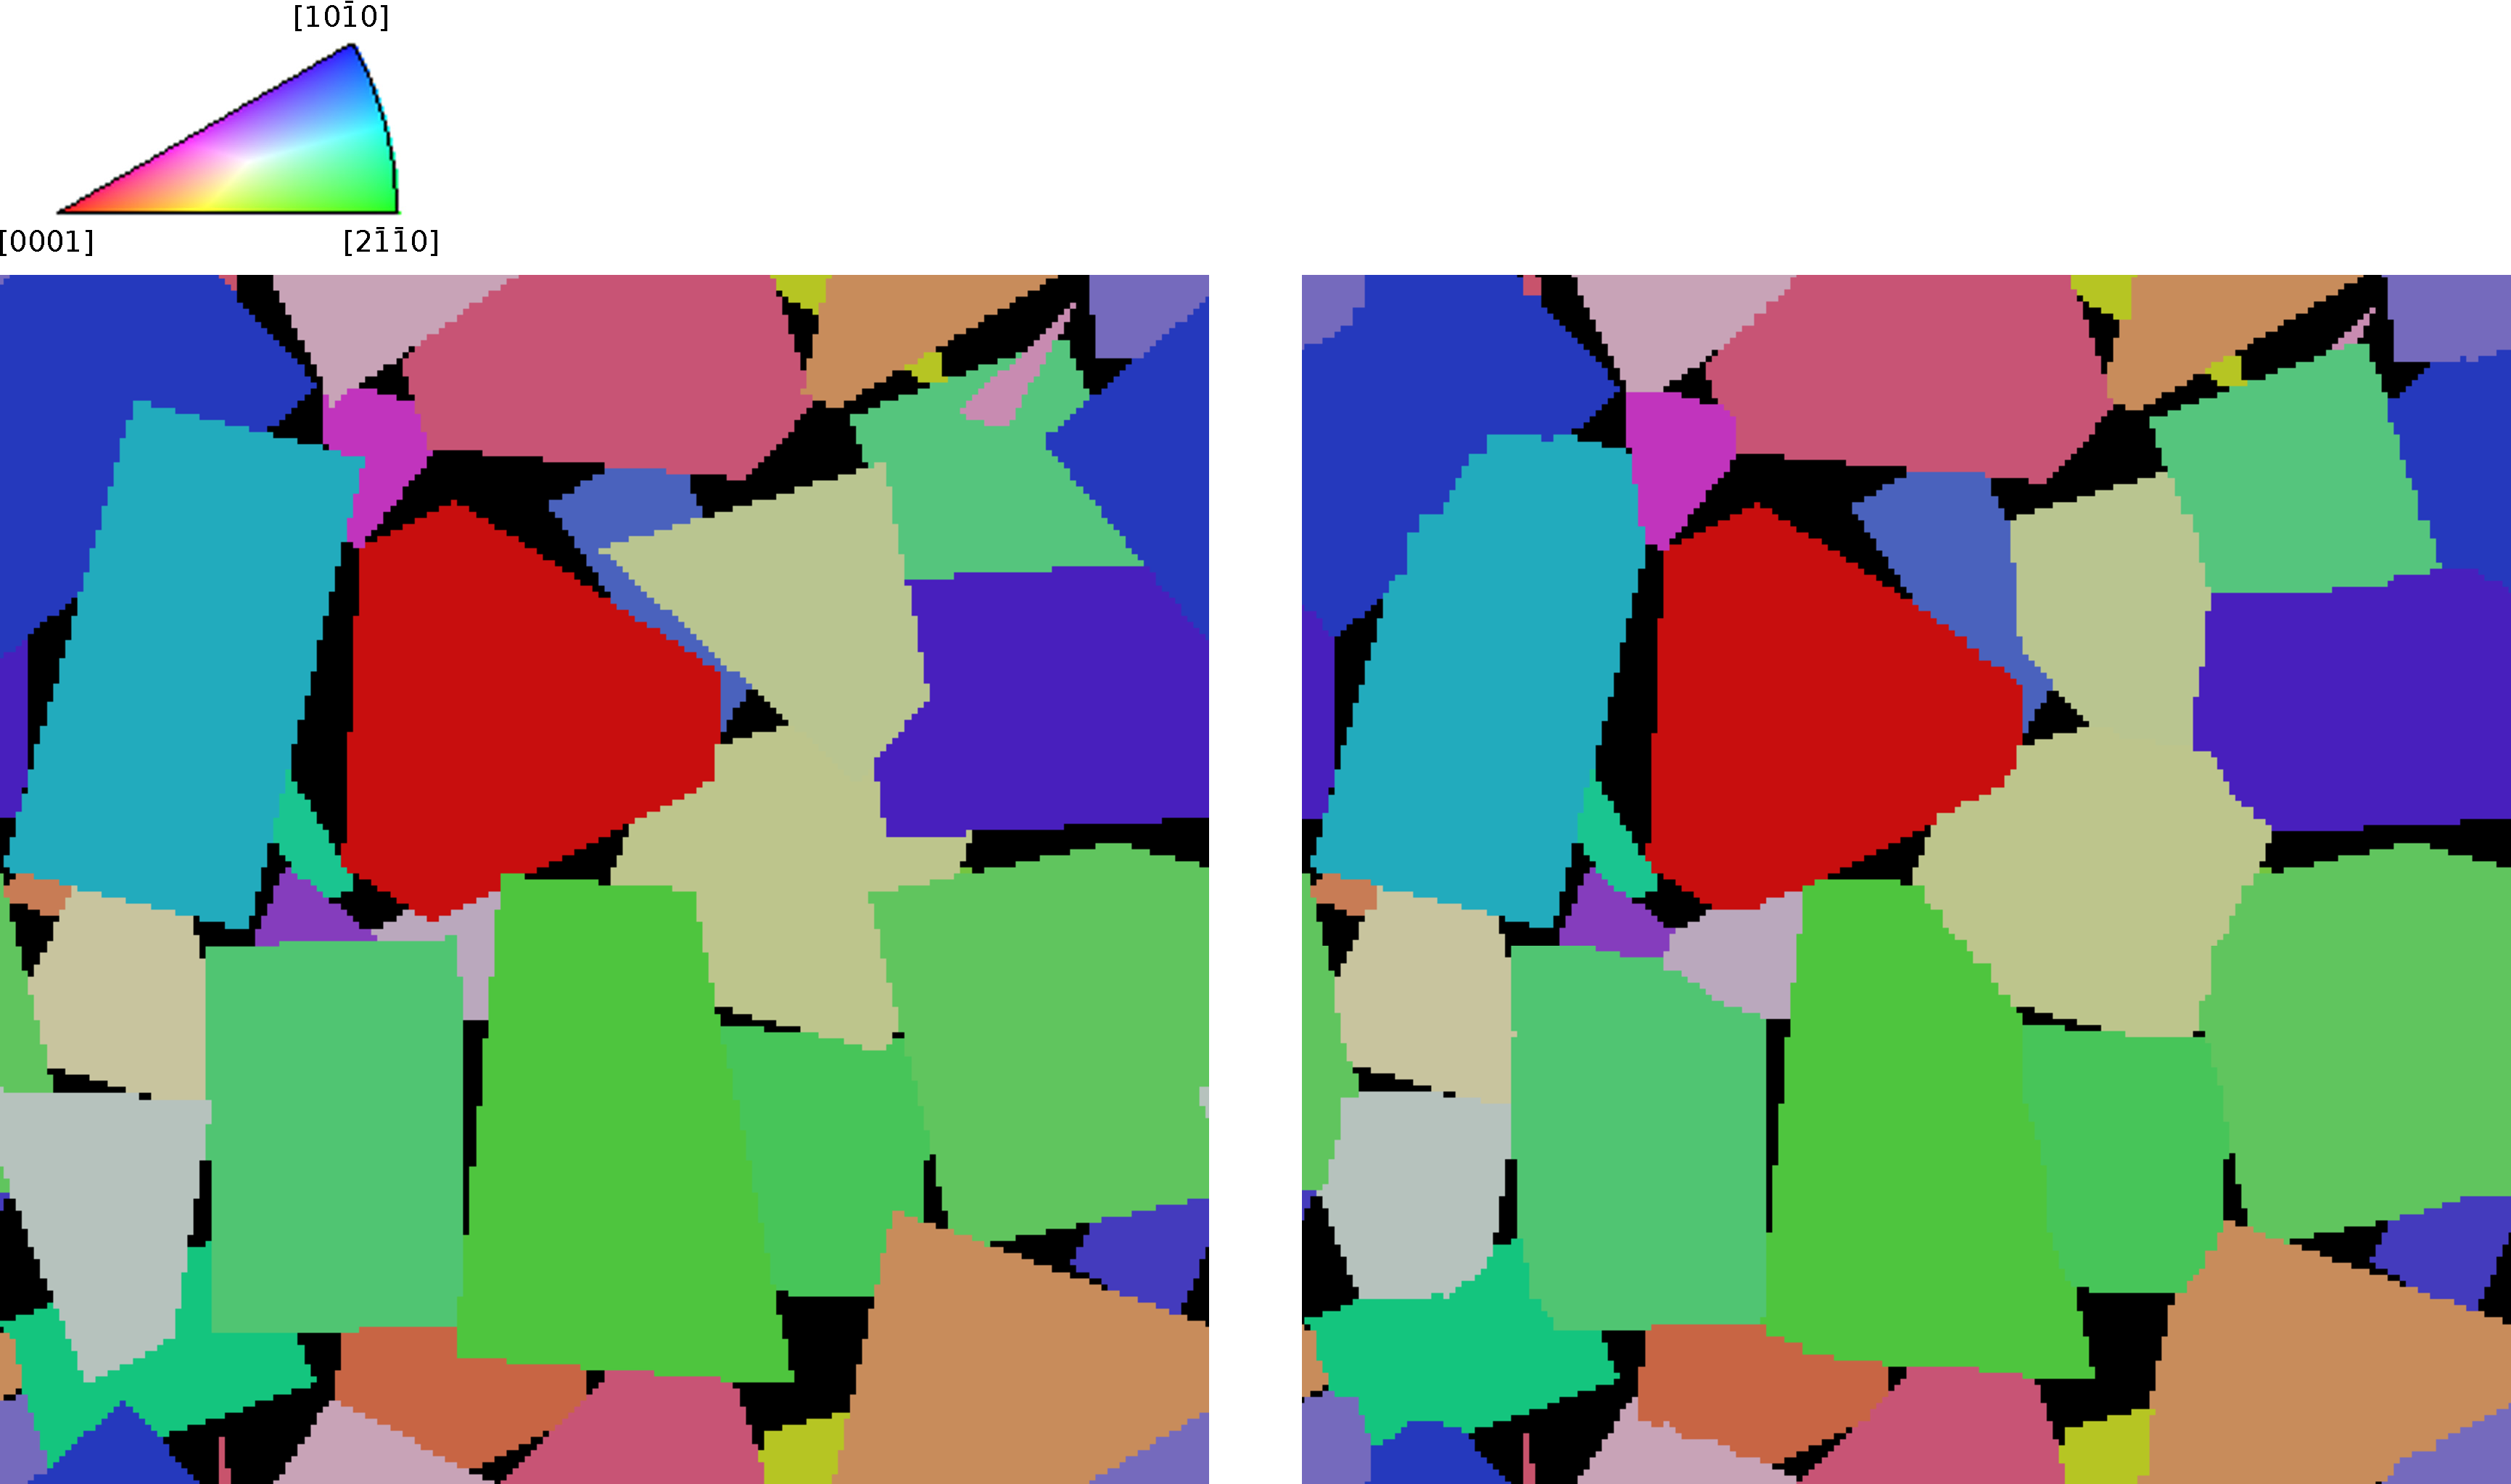
\includegraphics[width=\columnwidth]{Images/v105_slice1}
	\end{center}
	\caption{A slice of a generated microstructure before and after Potts simulation. The color coding corresponds to the orientation of the grains. The binder is black. The Co volume fraction is $0.098$ and the contiguity is $0.56$. The input parameters are $L=5 \, \mu\text{m}$, $M=200$, $r \in U[0.1, 0.4]$, $k \in U[0.6, 1.2]$, and $d_\text{eq} \in U[0.5, 2.0] \, \mu\text{m}$. In the random translation method, $\Delta$ is restricted so that a grain is moved maximally $2.0 \, \mu \text{m}$ in any direction and 5000 translations are tested for each grain. $4000 \cdot M^3$ MC iterations are made at a temperature of $0.5$.}
	\label{fig:microstructure_1}
\end{figure}

\begin{figure}
	\begin{center}
		\includegraphics[width=\columnwidth]{Images/v105_slice2}
	\end{center}
	\caption{The same generated microstructure as in Figure~\ref{fig:microstructure_1} in a different slice before and after Potts simulation.}
	\label{fig:microstructure_2}
\end{figure}

\begin{figure}
	\begin{center}
		\includegraphics[width=\columnwidth]{Images/v105_slice3}
	\end{center}
	\caption{The same generated microstructure as in Figure~\ref{fig:microstructure_1} in a different slice before and after Potts simulation.}
	\label{fig:microstructure_3}
\end{figure}

\begin{figure}
	\begin{center}
		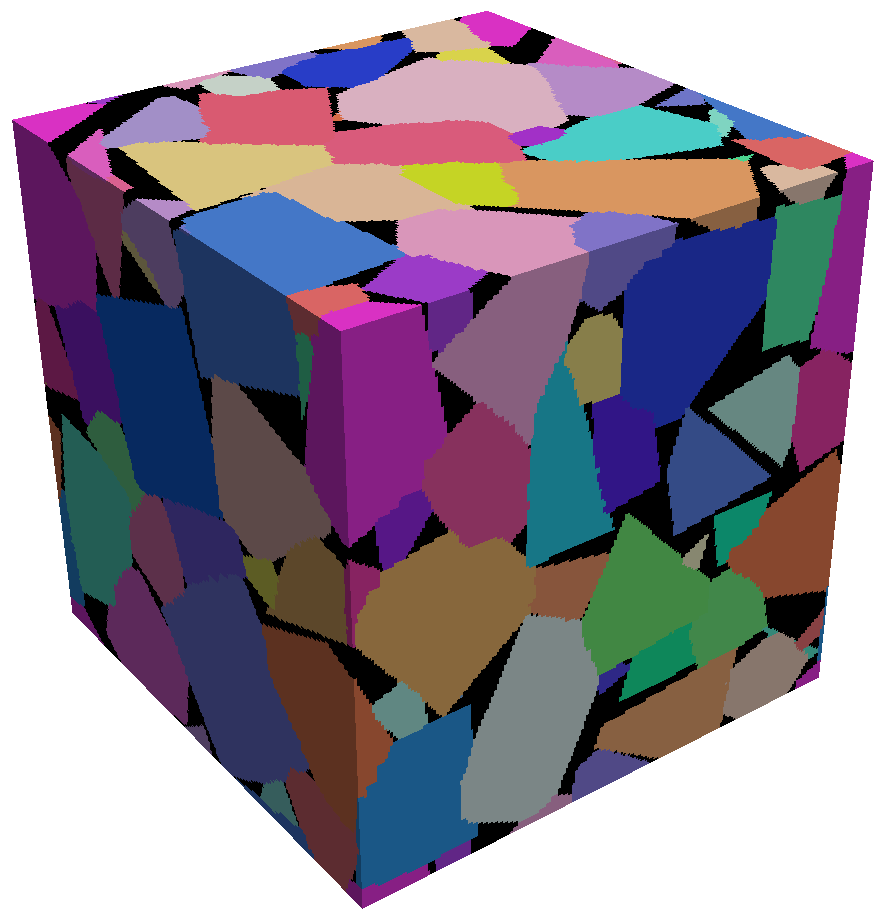
\includegraphics[width=.6\columnwidth]{Images/3D_view_e}
	\end{center}
	\caption{A 3D view of the surfaces of the same generated microstructure as in Figure~\ref{fig:microstructure_1} after Potts simulation.}
	\label{fig:microstructure_3d}
\end{figure}

\begin{figure}
	\begin{center}
		\includegraphics[width=\columnwidth]{Images/different_vol_frac}
	\end{center}
	\caption{Four generated microstructures after Potts simulation. The color coding corresponds to the orientation of the grains. The binder is black. The Co volume fractions are (from left to right, top to bottom) $0.124$, $0.152$, $0.183$, and $0.196$. The contiguities are $0.50$, $0.43$, $0.38$ and $0.34$. The input parameters are $L=5 \, \mu\text{m}$, $M=200$, $r \in U[0.1, 0.4]$, $k \in U[0.6, 1.2]$, and $d_\text{eq} \in U[0.5, 2.0] \, \mu\text{m}$. In the random translation method, $\Delta$ is restricted so that a grain is moved maximally $2.0 \, \mu \text{m}$ in any direction and 5000 translations are tested for each grain. $4000 \cdot M^3$ MC iterations are made at a temperature of $0.5$.}
	\label{fig:microstructure_diff_vol_frac}
\end{figure}

In Figure~\ref{fig:microstructure_grain_size_dist_1} and \ref{fig:microstructure_grain_size_dist_2}, the grain size distributions for two different Co volume fractions are plotted. Before placing the grains in the simulation volume, the grain sizes are drawn from a uniform distribution in the range $[0.5, 2.0] \, \mu\text{m}$. As seen, placing the grains in the volume shifts the distribution towards smaller grain size with more smaller grains for lower Co fraction. The Potts simulation levels out the distribution somewhat. To replicate an experimental distribution, a clever choice of initial distribution must be made.

\begin{figure}
	\begin{center}
		\includegraphics[width=\columnwidth]{Result_plots/runs2/grain_size_dist_17}
	\end{center}
	\caption{Average grain size distribution for 16 generated structures with $v_\text{Co} = 0.185$ and a total of $1281$ grains. The input parameters are $L=5 \, \mu\text{m}$, $M=200$, $r \in U[0.1, 0.4]$, $k \in U[0.6, 1.2]$, and $d_\text{eq} \in U[0.5, 2.0] \, \mu\text{m}$. In the random translation method, $\Delta$ is restricted so that a grain is moved maximally $2.0 \, \mu \text{m}$ in any direction and 5000 translations are tested for each grain. $4000 \cdot M^3$ MC iterations are made at a temperature of $0.5$.}
	\label{fig:microstructure_grain_size_dist_1}
\end{figure}

\begin{figure}
	\begin{center}
		\includegraphics[width=\columnwidth]{Result_plots/runs2/grain_size_dist_22}
	\end{center}
	\caption{Average grain size distribution for 16 generated structures with $v_\text{Co} = 0.083$ and a total of $1616$ grains. The input parameters are $L=5 \, \mu\text{m}$, $M=200$, $r \in U[0.1, 0.4]$, $k \in U[0.6, 1.2]$, and $d_\text{eq} \in U[0.5, 2.0] \, \mu\text{m}$. In the random translation method, $\Delta$ is restricted so that a grain is moved maximally $2.0 \, \mu \text{m}$ in any direction and 5000 translations are tested for each grain. $4000 \cdot M^3$ MC iterations are made at a temperature of $0.5$.}
	\label{fig:microstructure_grain_size_dist_2}
\end{figure}

\section{Discussion}

\begin{itemize}
	\item To replicate experimental grain size distributions, more work is needed to find a suitable initial size distribution.
	\item To obtain a contiguity curve in agreement with experiment also at high Co fraction, explicit inclusion of low-$\Sigma$ boundaries is needed. This can be achieved by inserting grains consisting of several sub-grains with low-$\Sigma$ intra-grain boundaries.
	\item The misorentiation across grain boundaries has not been examined and it is thus not known if it corresponds to a uniformly random distribution. Since grains are randomly translated to find minimum overlap, there is a risk of orientation correlations developing.
\end{itemize}

\section{Outlook}

\begin{itemize}
	\item The issue of meshing the generated structures for FEM analysis has not been touched upon in this report. It is our intention to use the surface meshing capabilites of Dream3D as a starting point for further body meshing, although this has not yet been tested.
	\item The Potts simulations are performed on a cubic grid and thus the voxels are cubic. By using instead an fcc grid, each voxel will have twelve instead of six neighbors. This can lead to smoother surfaces. Rather than improving CCBuilder, one could try to adapt some existing code for Potts simulations to give microstructures resembling WC-Co. The existence of good, parallellized code for Potts simulations has not yet been investigated.
% 	\item As an alternative to inserting grains of pre-defined shape, one could imagine running a true microstructure evolution simulation by applying the Potts model on all phases of the material with some seed particles. In that case, one would need to use orientation-dependent WC/Co interface energies to obtained faceted WC/Co interfaces. This would be an interesting alternative to more macroscopic grain growth simulations.
\end{itemize}


% Better control of grain size distribution. Look into experimental grain size distributions and try to replicate them better
% Explicit inclusion of low-Sigma boundaries. Intra-grain boundaries.
% Better implementation of Potts model, more connected lattice, e.g. fcc or adapting existing code for Potts model (parallelization)
% Potts model on all boundaries? WC/Co as well as WC/WC?
% Hope that Dream3D does surface meshing adequately


\bibliographystyle{elsart-num}
\bibliography{SyntheticStructure.bib}

\end{document}

